\justifying
\NSFCBodyText

\subsubsection{研究背景与意义}

预训练语料不再只是模型训练的被动原料，其组成会影响模型的知识边界、语言能力和计算效率。随着模型参数和训练预算增加，无差别扩充语料受到许可、重复、噪声和算力成本的共同限制。在既定计算条件下，哪些数据能够产生有效学习更新，因而成为语言模型从规模扩张转向数据机制研究时必须回答的问题。计算最优训练规律说明模型规模、训练 token 与性能之间存在系统约束\cite{trainingcomputeoptimal2022,scalinglanguagemodels2021,scalinglawsfor2020}，大规模语料工程也表明，来源选择、去重、过滤和混合方式能够影响训练过程与最终能力\cite{therefinedwebdataset2023,dolmaanopen2024,thefalconseries2023}。语料质量由此超出了预处理工程指标的范畴：它引起何种学习效应，这些效应在什么条件下成立，仍需专门研究。

目前常用的质量评价多依赖困惑度、表面规范性、来源声誉或与百科类“高质量文本”的相似程度。此类指标便于扩展到海量网页，却把不同性质的文本压缩到同一排序轴上。乱码、异常截断、段落错序等结构破损会削弱上下文的可学习关系；网络/地域书写、简繁异体或中英混写等结构完整但模型低熟悉的中文表达，也可能因困惑度较高或偏离规范语体而获得低分。两者的表面分数相近，训练含义却未必相同：修复前者可能减少与有效学习目标不一致的更新，删除后者则可能减少语体、实体和长尾知识的非冗余支持。若不区分这两种来源，“提高平均质量”便可能同时包含去除结构缺陷的收益和收缩语义支持的损失。

\begin{figure}[htbp]
  \centering
  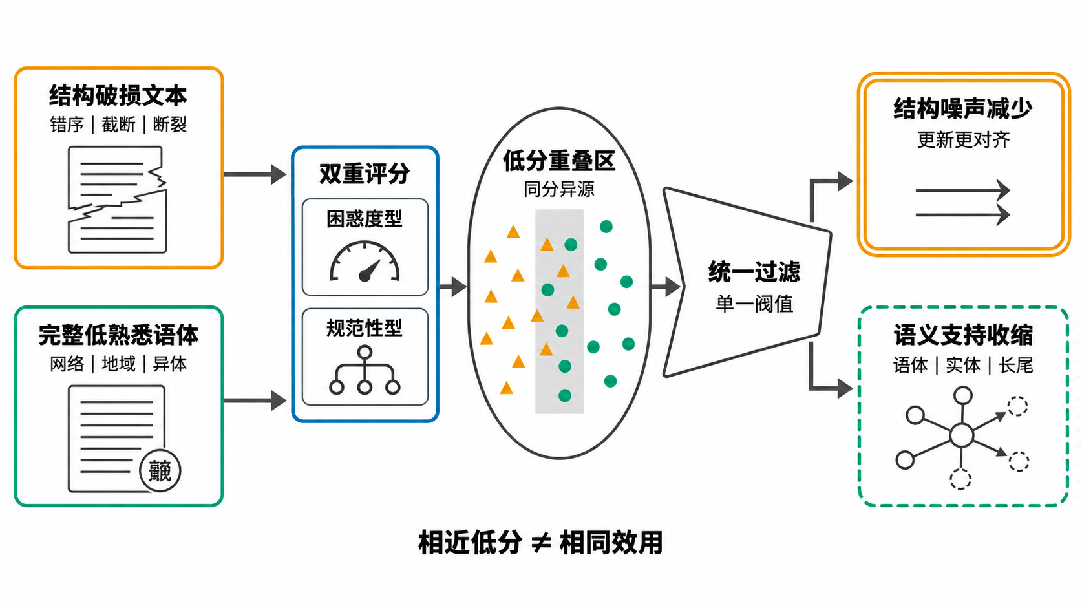
\includegraphics[width=0.98\linewidth]{figures/F01-background.pdf}
  \caption{相近低质量表征的异源构成及统一过滤悖论（概念示意）}
  \label{fig:background-paradox}
\end{figure}

这一矛盾在中文语料中尤为适合被严格检验。中文没有天然词间空格，简繁/异体、古今语体、网络表达和中英混写会共同影响 tokenizer 切分、序列长度、模型困惑度与规范性判断；表面“不熟悉”并不等同于语义破损。公开中文模型和评价基准已经为中文理解能力研究提供了可复核载体\cite{baichuanseedsharingthe2024,chatglmafamily2024,cmmlumeasuringmassive2024}，但多语言质量过滤研究也提示，跨语言评分需要显式处理语言差异，不能直接把英语网页中的质量经验平移到中文\cite{ali2025jql}。研究中文语料的意义因而不在于把现有筛选器换一批数据验证，而在于利用中文书写与语体异质性，检验“表面质量表征与训练效用是否等价”这一更一般的机制命题。

本项目聚焦公开可许可中文语料和小中规模开源自回归模型的受控继续预训练，不从零训练通用大模型，也不追求覆盖所有中文现象。项目拟预注册一类结构完整、来源可核验但模型低熟悉的中文语体作为确认性对象，并以另一类书写/语体现象作稳健性复核；通过可逆结构修复、sham 编辑、同语体非冗余支持补回、同语体窄支持补回和主流文本伪补回，分别定义结构缺陷削减与语义支持损失的反事实。若能说明相近低质量表征为何形成不同作用路径和反事实响应，就可把语料筛选研究从“哪个分数更准”推进到“分数背后的效用路径在何种条件下成立”，也为防止低频中文表达在自动过滤中被系统性排除提供可检验的理论依据。

\subsubsection{国内外研究现状及发展动态分析}

\paragraph{预训练语料工程已从规模构建转向质量策展，但质量对象仍常被混合。}

大规模开放语料的建设形成了网页抽取、语言识别、规则过滤、去重、来源记录和数据卡等基本流程。RefinedWeb、Dolma 等工作显示，经系统处理的网页语料可以支撑有竞争力的语言模型训练\cite{therefinedwebdataset2023,dolmaanopen2024}；数据审计研究则强调，仅知道语料规模不足以理解其组成和潜在偏差，需要追溯来源、内容类别与处理历史\cite{whatsin2023,anarchivalperspective2024}。去重研究证明，训练样本重复与模型记忆、过拟合及评价污染密切相关\cite{deduplicatingtrainingdata2022,quantifyingmemorizationacross2022}。这些研究奠定了“数据可治理”的基础，但文档完整性、集合多样性和特定模型上的边际效用分别属于文档级、集合级与模型条件层级，三者并不能由一个静态分数自然统一。

近年来的数据选择方法开始从单规则转向多维评分或多评价器协同。Meta-rater 组合多维信号评估预训练样本，Multi-Actor 通过多主体协作提高数据选择效率，FIRE 则研究多种质量评分的灵活整合\cite{zhuang2025metarater,bai2025multiactor,xu2025fire}。多语言质量判别进一步尝试缓解单一语言评分器的迁移问题\cite{ali2025jql}。这些进展提高了排序表达力，但其主要目标仍是预测或优化筛选结果。当结构破损与低频但有效的语体在评分空间中重叠时，增加评分器数量未必能解释两类样本为何具有不同训练效应。“怎样打分”已有较多探索，而“同一低分由何种机制产生、删除后果为何不同”仍缺少反事实证据。

\paragraph{质量过滤与多样性保持的矛盾已被认识，但现有结果不足以识别作用路径。}

数据选择研究已经注意到高质量、重要性和多样性之间不能相互替代。面向重要数据的多样性选择直接把覆盖纳入预训练样本选择\cite{harnessingdiversityfor2024}，网页重写等路线则尝试在不简单删除内容的情况下改善文本形态\cite{rephrasingtheweb2024}。MiniPile 等数据高效研究也说明，更小但经过选择的语料可以改变单位 token 收益\cite{theminipilechallenge2023}。因此，本项目不把“过滤会损失多样性”或“质量与覆盖存在权衡”作为创新结论；这些认识已构成研究背景。

尚未解决的是，现有工作多比较不同筛选策略或阈值产生的净效果。阈值提高会同时改变结构缺陷比例、来源构成、独立样本数、长尾覆盖和重复曝光，观察到的能力升降无法区分是缺陷减少、支持收缩、语体曝光变化，还是处理后重复训练轮次增加造成的。即使在相同 token 预算下，字符数、有效语义单元、packing 效率和数据处理成本也可能不同。缺少“保持支持只修复结构”和“保持语体曝光只改变非冗余广度”的正交反事实，质量收益与覆盖损失仍只是事后解释，不能形成可证伪的机制判断。

\paragraph{数据混合与动态重加权揭示模型条件效用，却难以替代机制识别。}

DoReMi、DoGE 和数据混合律等工作以代理模型或验证目标优化领域配比，表明最优数据组合依赖目标分布和模型条件\cite{doremioptimizingdata2023,dogedomainreweighting2023,datamixinglaws2024}。Skill-it! 从技能依赖出发组织数据，ScaleBiO 等方法则将预训练数据重加权写成可扩展的双层优化问题\cite{skillita2023,scalebioscalablebilevel2024}。自影响重加权和动态损失重加权进一步说明，样本价值随训练状态和评价目标变化，固定排序不是唯一合理选择\cite{selfinfluenceguided2023,dynamiclossbased2025}。

这条路线说明数据效用取决于具体条件，同时留下两个问题。第一，数据混合方法通常以验证损失或聚合能力为优化目标，容易把机制不同的样本统一解释为权重差异；它可以找到更有效的组合，却未必回答结构修复与语义支持恢复为何产生差异。第二，代理模型上得到的领域权重、排序或阈值会受到模型规模、tokenizer 和基础训练史影响，直接外推存在风险。本项目据此把处理前模型知识状态作为双路径效应的边界条件，不另行开发动态选样算法。只有从共同 checkpoint 随机分叉，才能区分状态调节与处理后的路径依赖。

\paragraph{训练数据影响分析提供了机制读出，但相关性不能自动成为因果中介。}

训练数据影响与估值研究尝试追踪单个样本或数据子集对模型输出的贡献，包括自影响、影响函数、事实追踪和免训练估值等路线\cite{trainingdatainfluence2024,whatisyour2025,scalableinfluenceand2024,datavaluationwithout2023,opendatavalaunified2023}。这些方法为观察“某批数据的更新朝向何处”提供了工具，也暴露出计算开销、目标依赖和尺度迁移等限制。训练数据抽取研究表明，模型可能保留可被抽取的训练记忆；这要求能力评价进一步排除训练—评价近邻和污染，不能把可复现答案直接视为一般知识吸收\cite{extractingtrainingdata2020,scalableextractionof2023}。

对本项目而言，原始损失更低不一定表示样本更有用，梯度方差更大也可能同时来自有价值的新信息和有害结构噪声。为降低事后选择自由度，本项目只把“能力定向梯度对齐”作为主动力学读出，即在固定 probe 上度量训练 batch 梯度与独立能力诊断集梯度的单位 token 归一化方向关系。该读出仍只是局部候选中介：只有处理先改变读出，读出对后续独立能力有留出预测增益，并且修复/恢复时读出与能力共同逆转，才支持动力学中介解释。仅凭加入中介变量后回归系数改变，不足以声称机制成立。

\paragraph{中文场景具备研究基础，但“使用中文数据”本身不是创新。}

中文开放模型、语料构建和多任务评价的发展，使得受控继续预训练与中文能力测量成为可执行研究对象\cite{baichuanseedsharingthe2024,chatglmafamily2024,cmmlumeasuringmassive2024}。与此同时，基准可能受污染、反复调参和构念覆盖不足影响，单一榜单不能代表语体、知识与长尾能力\cite{inadequaciesoflarge2024}。多语言筛选工作证明语言条件需要进入质量评价\cite{ali2025jql}，但尚不能回答中文内部的表面规范性、模型熟悉度和语义完整性如何共同塑造训练效用。

中文语料在本项目中构成一项压力测试：结构完整的低频中文语体与真正结构破损的文本可能被静态质量表征压缩为相近低分，但两者分别关联可学习的非冗余支持与低目标对齐更新。确认这一点需要至少两类异质评分器、人工语义完整性审查以及独立能力终点，单个自建分类器不足以支持判断。所得结论限于预注册中文语体、公开数据来源和小中规模继续预训练条件，不预设该机制为中文独有。

\subsubsection{现有研究的不足}

综上，现有工作已经证明数据处理会影响预训练结果，也形成了质量评分、多样性选择、数据混合和影响估计等丰富方法，但仍存在三项相互关联的认知缺口。

第一，\textbf{静态低质量表征的效用异质性缺少可干预解释}。结构破损与模型低熟悉的完整中文语体可能获得相近分数，现有筛选对比却难以说明两类低分样本的效用为何不同。若只提高分类准确率或组合更多指标，仍可能把评分器的测量偏差当作数据质量机制。

第二，\textbf{缺陷削减与语义支持损失缺少路径特异的反事实证据}。常规过滤同时改变质量、语体比例、非冗余广度和曝光次数；观察到强过滤后能力下降，并不能证明原因是覆盖损失。同语体非冗余补回是否优于同语体重复/窄支持补回和主流文本补回，是区分“非冗余支持”“语体曝光”与“等量补数”的关键反证，但尚少有研究在受控继续预训练中同时设置这些对照。

第三，\textbf{两条路径的动力学证据和适用边界尚不清楚}。梯度、损失和遗忘指标可能都与最终能力相关，却处于不同统计层级；把大量 token 或 checkpoint 当作独立样本会产生伪重复。来源和模型状态变化还可能使效应反号。需要以训练运行为推断单位，冻结主读出和能力终点，并在独立来源中检验效应方向、预测区间和拒绝外推条件。

这三项缺口依次涉及低分来源、作用路径和适用边界：先识别两类低分来源，再用特异恢复和负对照分离作用路径，最后检验路径效应能否跨来源保持以及何时失效。三者共同指向同一个机制问题。

\subsubsection{关键科学问题与研究切入点}

本项目拟回答的中心科学问题是：\textbf{中文语料中，结构破损文本与结构完整但模型低熟悉的中文语体为何会获得相近的低质量表征，却经由结构缺陷削减和非冗余语义支持损失形成不同作用路径与反事实响应；这种效用异质性如何受模型既有知识状态调节？}

围绕该问题提出如下可证伪假设：\textbf{中文语料的静态低质量表征混合了结构缺陷与低模型熟悉度两类成分。结构破损产生与有效学习目标低对齐的更新；结构完整但模型低熟悉的中文语体可提供面向相应能力的非冗余更新。因此，保持语义支持的结构修复应提高训练更新的能力定向梯度对齐并改善通用能力；保持语体曝光量的非冗余支持补回应选择性改善语体与长尾能力。前一路径检验结构损伤及恢复，后一路径检验移除后的支持补回；二者共同解释低质量表征的效用异质性，不把两个估计量直接解释为同一种过滤效应的方向比较。}

该假设允许被直接否定：在分词与 packing、总 token、语体曝光量及训练—评价重叠受控后，若原文恢复相对 sham 编辑不能提高能力定向梯度对齐和独立后测能力，则结构路径被否定；若同语体非冗余补回不优于同语体等量重复/窄支持补回及主流文本补回，则语义支持路径被否定。任一路径失败均不以“状态依赖”或重新校准作兜底解释。

本项目从评分、干预、动力学与能力四个层级切入，不另行构造综合质量分。首先用两类异质质量表征和人工盲审定位“分数重叠而生成机制不同”的样本层；继而以可逆结构破损、原文恢复和 sham 编辑识别结构路径，以同语体非冗余、同语体窄支持和主流文本补回识别支持路径；最后通过共同 checkpoint 随机分叉和独立来源的冻结协议复核模型状态与外部边界。即使这些实验没有产生更好的过滤策略，反证结果仍能回答两类效应是否存在、哪些替代机制可以解释效应以及结论能否外推。
